\chapter{Solution}
The figure \ref{fig:flow} shows the flow diagram of hand gesture recognition system that is going to implemented in this thesis. Each block contains different software components that are executed sequentially. However, training phase must be carried out before this system is available for recognition. Finally, these components will be integrated into NAO.

\begin{figure}
	[!h] \centering 
	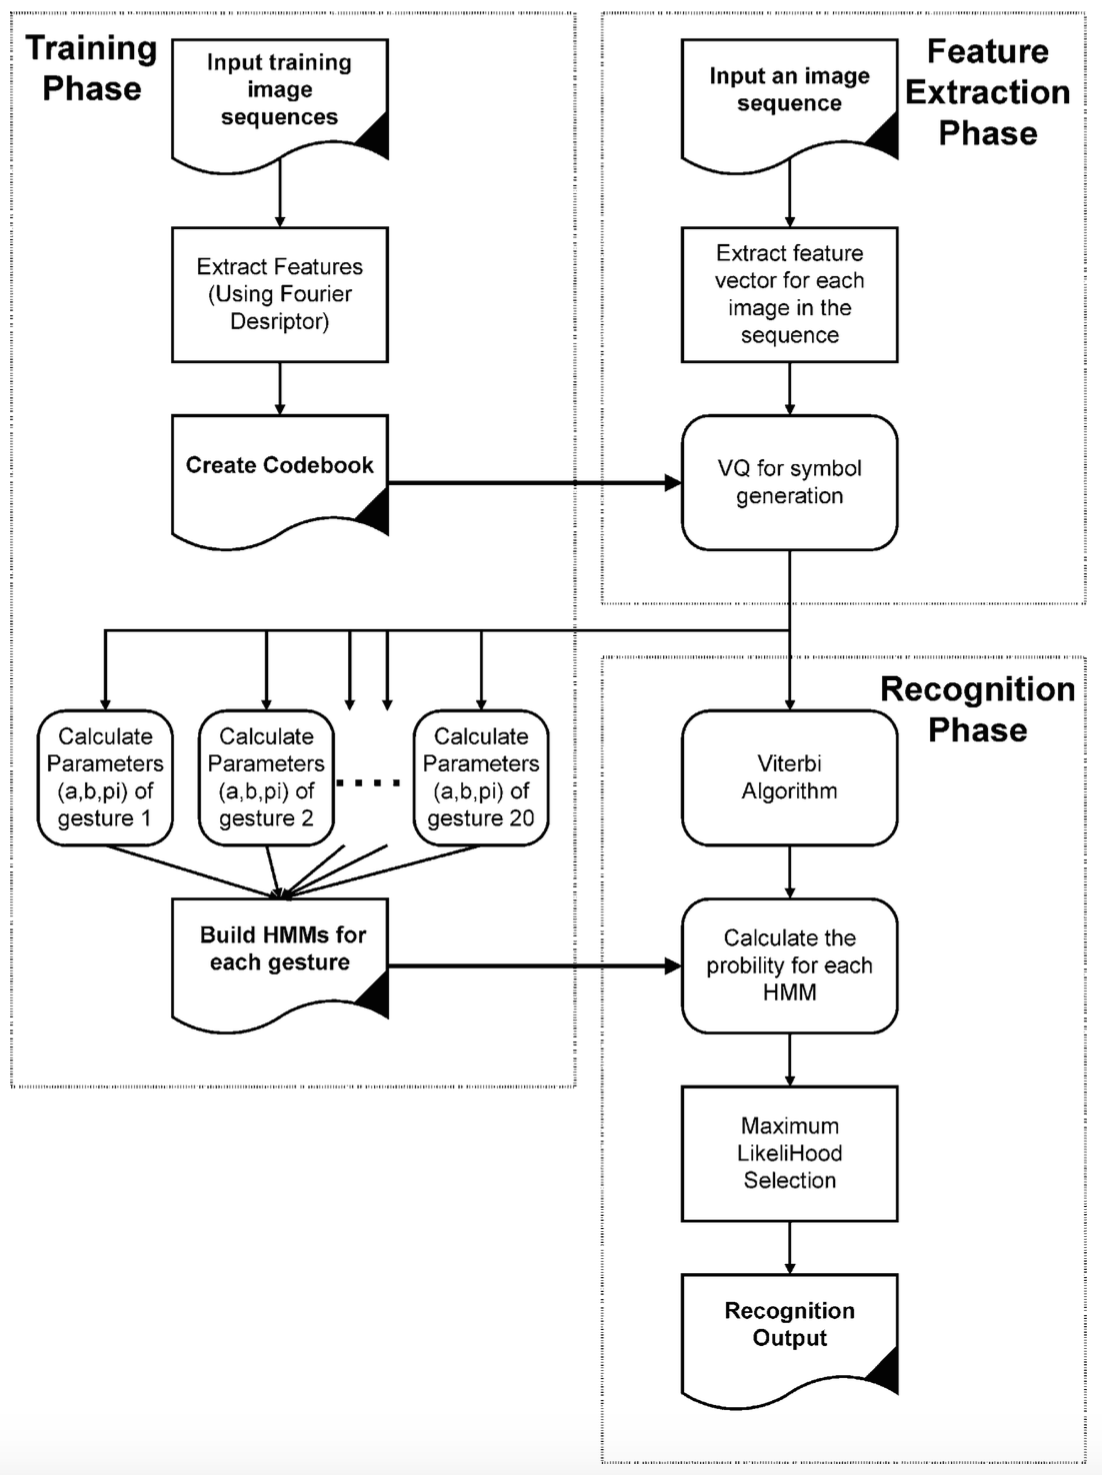
\includegraphics[width=9cm]{figures/flow.png} \caption{Flow diagram of hand gesture recognition system \cite{5}.} \label{fig:flow} 
\end{figure}

\section{Sensing} 
3D camera records 30 frames of color image as well as depth image per second and outputs as a data package. Figure \ref{fig:depth} shows the single frame of depth image taken from Microsoft Kinect where darker gray values represent the farther distance and lighter gray values represent the closer distance from the camera.

\begin{figure}
	\centering
	\begin{minipage}{.5\textwidth}
		\centering
		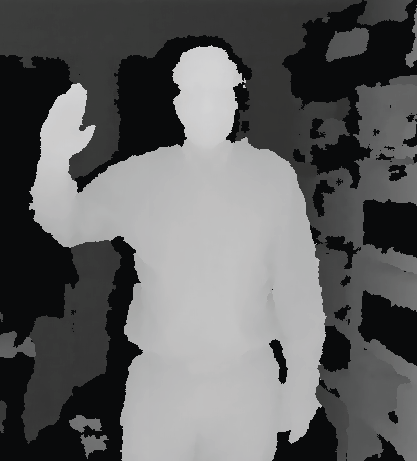
\includegraphics[height=7cm]{figures/depth.png} 
		\captionof{figure}{Depth image from 3D Camera}
		\label{fig:depth}
	\end{minipage}%
	\begin{minipage}{.5\textwidth}
		\centering
		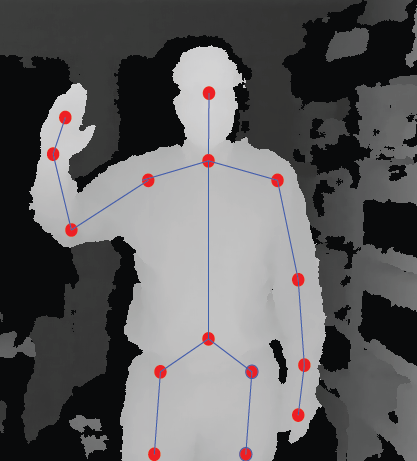
\includegraphics[height=7cm]{figures/depth-skeleton.png}
		\captionof{figure}{Skeleton tracking}
		\label{fig:skeleton}
	\end{minipage}
\end{figure}

\section{Feature Extraction}
Output package from sensor data will be inputted to feature detection and extraction unit. OpenNI is a software component that will track the anatomical landmarks of the human body from the package and extract significant joint angle parameters along with segment length and present them three dimensionally as shown in the figure \ref{fig:skeleton}. Finally, only joints of both the arms will be picked out from the array of features, since it will be the significant joints needed for hand gesture recognition.

\section{Modeling and Classification}
In order to use this hand recognition system, all chosen gestures must be observed and the system must be trained. Therefore, a set of simple gestures will be chosen and observed for training. Each gesture is isolated in time and gesticulated for certain duration. However, sensors provides 30 frames of discrete states of gesture per second. 

For example, a gesture is gesticulated by simply drawing a circle in the air and its ideal states are shown in the figure \ref{fig:ges:state}. It will be  as a position of hand passing through 8 states of the circle. Each state is a point in space with x, y and z axis data. This approach makes it possible for us to reduce our observation data to sequential 3D points and focus on the recognition task without processing all those pixels. Each trained model can then be used to determine with what probability a given gesture appears in test data. Therefore, the trained Hidden Markov models will be used to recognize gestures \cite{2}. 

\begin{figure}
	\centering
	\begin{minipage}{.3\textwidth}
		\centering
		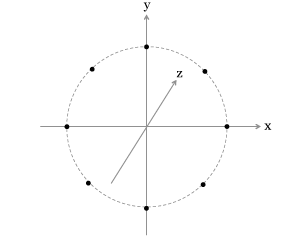
\includegraphics[width=6cm]{figures/ges-states.png}
		\captionof{figure}{HMM States of circular gesture \cite{9}.}
		\label{fig:ges:state}
	\end{minipage}%
	\begin{minipage}{.7\textwidth}
		\centering
		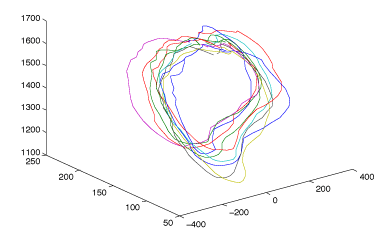
\includegraphics[width=10cm]{figures/ges-train.png}
		\captionof{figure}{Observations of a circular gesture in x, y, z axis which are recorded by a depth camera \cite{9}.}
		\label{fig:ges:train}
	\end{minipage}
\end{figure}

\section{Gesture Analysis and Recognition}
This step contains the analysis of gesticulated gesture and finding out the likelihood of that gesture with trained data, known as gesture recognition. Figure \ref{fig:ges:train}  contains colored rings of noisy data of gestures that represent instances of a real circle gesture. Sensing and feature detection module will produce 60 observations of the circle gesture for 2 seconds, since the depth camera records at 30 frame per second. To decide whether a given set of 60 observations contains a circle gesture, we need to first determine the likelihood that the hand passed through the eight states of the gesture in the expected sequence.

Discrete HMM is a finite set of possible output symbols and a sequence of hidden states which reveal some probability. To reduce our real gesture data to a workable number of discrete output symbols and states, we can use any clustering algorithm to cluster the 3D points of all our training data of circle gesture into clusters and label them. That is to say, every point in the training data represents an output symbol that is closely tied to one of the 8 true states of the model.

Looking at the labeled data, we can estimate how likely it is that a hand passed through the 8 clusters in the same sequence as a circle gesture and if the likelihood is high enough, then the gesture is considered to be recognized.

\begin{figure}
	[h] \centering 
	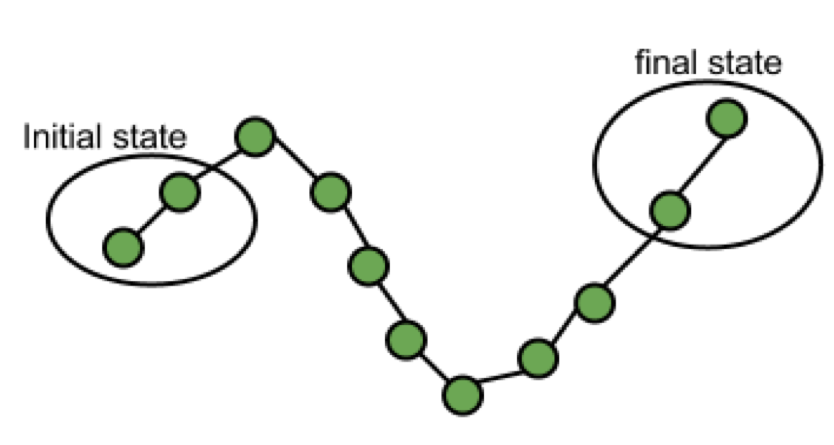
\includegraphics[height=7cm]{figures/ges-rec.png} \caption{The states of Arabic sign language to convey "Hello" \cite{11}. It is consisted of 11 states of Markov models and if there is higher likelihood of the hand position passed through states sequentially from initial to final, then it is recognized as "Hello".} \label{fig:ges:reg} 
\end{figure}

\section{Human-Robot Interaction}
Finally, the recognized gesture will be interpreted by NAO to execute a specified task. For example. circle gesture would ask NAO to turn around. However, NAO will also be available in Translation Mode by using ALTextToSpeech Library to translate the recognized gesture.

